\documentclass[10pt,a4paper]{article}
\usepackage[utf8]{inputenc}
\usepackage[T1]{fontenc}
\usepackage[left=0.30in, right=0.30in, top=0.24in, bottom=0.24in]{geometry}
\usepackage{graphicx}
\usepackage{booktabs}
\usepackage{xcolor}
\usepackage{colortbl}
\usepackage{tabularx}
\usepackage{tcolorbox}
\usepackage{titlesec}
\usepackage{microtype}
\usepackage{helvet}
\usepackage{amsmath,amssymb}
\usepackage{enumitem}
\usepackage{hyperref}

\renewcommand{\familydefault}{\sfdefault}
\pagestyle{empty}

% Institutional Color Palette (Athénée Investment)
\definecolor{primary}{RGB}{15, 23, 42}       % Deep Institutional Navy
\definecolor{accent}{RGB}{26, 54, 93}        % Royal Slate Navy
\definecolor{goldaccent}{RGB}{176, 138, 87}  % Athénée Warm Bronze/Gold
\definecolor{cardbg}{RGB}{248, 250, 252}     % Crisp Light Slate Background
\definecolor{cardborder}{RGB}{218, 226, 236} % Subtle Card Border
\definecolor{posgreen}{RGB}{34, 197, 94}     % Positive Return Green
\definecolor{negred}{RGB}{239, 68, 68}       % Negative Return Red
\definecolor{mutedtext}{RGB}{100, 116, 139}  % Secondary Slate Text

\hypersetup{
    colorlinks=true,
    linkcolor=accent,
    urlcolor=accent
}

\tcbuselibrary{skins}

\begin{document}

%%%%%%%%%%%%%%%%%%%%%%%%%%%%%%%%%%%%%%%%%%%%%%%%%%%%%%%%%%%%%%%%%%%%%%%%%%%%%%%
%% PAGE 1: INSTITUTIONAL ONE-PAGER TEAR SHEET
%%%%%%%%%%%%%%%%%%%%%%%%%%%%%%%%%%%%%%%%%%%%%%%%%%%%%%%%%%%%%%%%%%%%%%%%%%%%%%%

% --- HEADER BAR WITH LOGO ---
\noindent
\begin{minipage}[c]{0.69\textwidth}
    {\fontsize{19}{23}\selectfont \bfseries \textcolor{primary}{Valais Citadel (ATH-804)}}\\[2.5pt]
    {\small \bfseries \textcolor{accent}{Systematic Global Macro Strategy}}\\[3pt]
    {\footnotesize \textcolor{primary}{\textbf{Track Record: Jan 2010 -- Jun 2026}} \ \textcolor{goldaccent}{\textbf{(198 Months / 16.5 Years)}} \quad $\vert$ \quad \textcolor{mutedtext}{\textbf{Benchmark:} S\&P 500 Total Return}}
\end{minipage}%
\hfill
\begin{minipage}[c]{0.29\textwidth}
    \raggedleft
    
\includegraphics[height=1.08cm, keepaspectratio]{athenee_logo.png}\\[1.5pt]
    {\tiny \bfseries \textcolor{goldaccent}{CAPITAL INTRODUCTION \& THIRD-PARTY MARKETING}}
\end{minipage}

\vspace{0.22em}
\noindent{\color{goldaccent}\rule{\textwidth}{1.4pt}}
\vspace{0.25em}

% --- SECTION 1: 6 TOP-LINE KPI HIGHLIGHT CARDS (INCL. DEDICATED ALPHA BOX + BETA & CORR BOX) ---
\noindent
\begin{tcolorbox}[nobeforeafter, box align=top, width=0.160\textwidth, colback=white, colframe=primary, title=\textbf{\scriptsize\strut CAGR (Net)}, fonttitle=\sffamily\bfseries\scriptsize, arc=4pt, boxrule=0.8pt, toptitle=3pt, bottomtitle=3pt, left=1.5pt, right=1.5pt, top=3.5pt, bottom=3.5pt, colbacktitle=primary, halign title=center]
    \centering
    {\large \bfseries \textcolor{primary}{\strut 21.69\%}}\\[1.5pt]
    {\tiny \textcolor{mutedtext}{\strut S\&P 500: 14.34\%}}
\end{tcolorbox}\hfill
\begin{tcolorbox}[nobeforeafter, box align=top, width=0.160\textwidth, colback=white, colframe=primary, title=\textbf{\scriptsize\strut Ann. Volatility}, fonttitle=\sffamily\bfseries\scriptsize, arc=4pt, boxrule=0.8pt, toptitle=3pt, bottomtitle=3pt, left=1.5pt, right=1.5pt, top=3.5pt, bottom=3.5pt, colbacktitle=primary, halign title=center]
    \centering
    {\large \bfseries \textcolor{primary}{\strut 7.20\%}}\\[1.5pt]
    {\tiny \textcolor{mutedtext}{\strut S\&P 500: 14.46\%}}
\end{tcolorbox}\hfill
\begin{tcolorbox}[nobeforeafter, box align=top, width=0.160\textwidth, colback=white, colframe=primary, title=\textbf{\scriptsize\strut Sharpe Ratio}, fonttitle=\sffamily\bfseries\scriptsize, arc=4pt, boxrule=0.8pt, toptitle=3pt, bottomtitle=3pt, left=1.5pt, right=1.5pt, top=3.5pt, bottom=3.5pt, colbacktitle=primary, halign title=center]
    \centering
    {\large \bfseries \textcolor{primary}{\strut 2.78}}\\[1.5pt]
    {\tiny \textcolor{mutedtext}{\strut SPX: 1.00 $\vert$ Sortino: 7.42}}
\end{tcolorbox}\hfill
\begin{tcolorbox}[nobeforeafter, box align=top, width=0.160\textwidth, colback=white, colframe=primary, title=\textbf{\scriptsize\strut Max Drawdown}, fonttitle=\sffamily\bfseries\scriptsize, arc=4pt, boxrule=0.8pt, toptitle=3pt, bottomtitle=3pt, left=1.5pt, right=1.5pt, top=3.5pt, bottom=3.5pt, colbacktitle=primary, halign title=center]
    \centering
    {\large \bfseries \textcolor{primary}{\strut -7.74\%}}\\[1.5pt]
    {\tiny \textcolor{mutedtext}{\strut SPX: -23.87\% $\vert$ Calmar: 2.80}}
\end{tcolorbox}\hfill
\begin{tcolorbox}[nobeforeafter, box align=top, width=0.160\textwidth, colback=white, colframe=primary, title=\textbf{\scriptsize\strut Alpha (Ann.)}, fonttitle=\sffamily\bfseries\scriptsize, arc=4pt, boxrule=0.8pt, toptitle=3pt, bottomtitle=3pt, left=1.5pt, right=1.5pt, top=3.5pt, bottom=3.5pt, colbacktitle=primary, halign title=center]
    \centering
    {\large \bfseries \textcolor{primary}{\strut 18.04\%}}\\[1.5pt]
    {\tiny \textcolor{mutedtext}{\strut $t$-stat: 10.14}}
\end{tcolorbox}\hfill
\begin{tcolorbox}[nobeforeafter, box align=top, width=0.160\textwidth, colback=white, colframe=primary, title=\textbf{\scriptsize\strut Beta \& Corr.}, fonttitle=\sffamily\bfseries\scriptsize, arc=4pt, boxrule=0.8pt, toptitle=3pt, bottomtitle=3pt, left=1.5pt, right=1.5pt, top=3.5pt, bottom=3.5pt, colbacktitle=primary, halign title=center]
    \centering
    {\large \bfseries \textcolor{primary}{\strut 0.14 $\vert$ +0.28}}\\[1.5pt]
    {\tiny \textcolor{mutedtext}{\strut Beta $t$-stat: 4.04}}
\end{tcolorbox}

\vspace{0.25em}

% --- SECTION 2: COMPREHENSIVE SINGLE-FUND ANALYSIS INDICATORS (STRICTLY ALIGNED 13 ROWS EACH) ---
\noindent
\begin{tcolorbox}[nobeforeafter, box align=top, width=0.492\textwidth, colback=white, colframe=primary, title=\textbf{\small\strut Performance, Risk \& Hit Rate Indicators}, fonttitle=\sffamily\bfseries\small, arc=5pt, boxrule=0.9pt, toptitle=3.5pt, bottomtitle=3.5pt, left=4pt, right=4pt, top=1pt, bottom=1pt, colbacktitle=primary]
\renewcommand{\arraystretch}{1.13}
\setlength{\tabcolsep}{2pt}
\scriptsize
\begin{tabular*}{\textwidth}{@{\extracolsep{\fill}} l r r @{}}
\rowcolor{primary!10!white}[0pt][0pt] \textbf{\textcolor{primary}{\strut Indicator}} & \textbf{\textcolor{primary}{\strut Fund}} & \textbf{\textcolor{mutedtext}{\strut S\&P 500}} \\
\textbf{\textcolor{primary}{\strut CAGR (Annualized)}} & \textbf{\textcolor{primary}{21.69\%}} & \textcolor{mutedtext}{14.34\%} \\
\rowcolor{cardbg}[0pt][0pt] \textbf{\textcolor{primary}{\strut Annualized Mean Return}} & \textcolor{primary}{20.04\%} & \textcolor{mutedtext}{14.52\%} \\
\textbf{\textcolor{primary}{\strut Annualized Volatility}} & \textcolor{primary}{7.20\%} & \textcolor{mutedtext}{14.46\%} \\
\rowcolor{cardbg}[0pt][0pt] \textbf{\textcolor{primary}{\strut Proxy Sharpe Ratio ($r_f = 0\%$)}} & \textbf{\textcolor{primary}{2.78}} & \textcolor{mutedtext}{1.00} \\
\textbf{\textcolor{primary}{\strut Annualized Sortino Ratio}} & \textcolor{primary}{7.42} & \textcolor{mutedtext}{1.66} \\
\rowcolor{cardbg}[0pt][0pt] \textbf{\textcolor{primary}{\strut Maximum Drawdown (MDD)}} & \textbf{\textcolor{primary}{-7.74\%}} & \textcolor{mutedtext}{-23.87\%} \\
\textbf{\textcolor{primary}{\strut Calmar Ratio (CAGR / $|$MDD$|$)}} & \textcolor{primary}{2.80} & \textcolor{mutedtext}{0.60} \\
\rowcolor{cardbg}[0pt][0pt] \textbf{\textcolor{primary}{\strut Cumulative Total Return}} & \textcolor{primary}{2451.43\%} & \textcolor{mutedtext}{812.87\%} \\
\textbf{\textcolor{primary}{\strut Best / Worst Monthly}} & \textcolor{primary}{+12.56\% / -5.07\%} & \textcolor{mutedtext}{+12.82\% / -12.35\%} \\
\rowcolor{cardbg}[0pt][0pt] \textbf{\textcolor{primary}{\strut Positive Months (Hit Rate)}} & \textcolor{primary}{86.9\% (172/198)} & \textcolor{mutedtext}{68.7\% (136/198)} \\
\textbf{\textcolor{primary}{\strut Crisis Hit Rate ($\text{Fund}>0 \mid \text{SPX}<0$)}} & \textbf{\textcolor{primary}{75.8\% (47/62)}} & \textcolor{mutedtext}{--} \\
\rowcolor{cardbg}[0pt][0pt] \textbf{\textcolor{primary}{\strut Up-Mkt Loss ($\text{Fund}<0 \mid \text{SPX}>0$)}} & \textcolor{primary}{8.1\% (11/136)} & \textcolor{mutedtext}{--} \\
\end{tabular*}
\end{tcolorbox}\hfill
\begin{tcolorbox}[nobeforeafter, box align=top, width=0.492\textwidth, colback=white, colframe=primary, title=\textbf{\small\strut Alpha, Beta, Correlation \& Tail Analysis (vs. S\&P 500)}, fonttitle=\sffamily\bfseries\small, arc=5pt, boxrule=0.9pt, toptitle=3.5pt, bottomtitle=3.5pt, left=4pt, right=4pt, top=1pt, bottom=1pt, colbacktitle=primary]
\renewcommand{\arraystretch}{1.13}
\setlength{\tabcolsep}{2pt}
\scriptsize
\begin{tabular*}{\textwidth}{@{\extracolsep{\fill}} l r @{}}
\rowcolor{primary!10!white}[0pt][0pt] \textbf{\textcolor{primary}{\strut Quantitative Metric}} & \textbf{\textcolor{primary}{\strut Estimate / Diagnostic}} \\
\textbf{\textcolor{primary}{\strut Annualized Alpha ($\alpha$) \& $t$-stat}} & \textbf{\textcolor{primary}{18.04\% (t=10.14)}} \\
\rowcolor{cardbg}[0pt][0pt] \textbf{\textcolor{primary}{\strut Market Beta ($\beta_{\text{SPX}}$) \& $t$-stat}} & \textcolor{primary}{0.14 (t=4.04) ($R^2=7.7\%$)} \\
\textbf{\textcolor{primary}{\strut Pearson Correlation ($r$) to S\&P 500}} & \textbf{\textcolor{primary}{+0.28}} \textcolor{mutedtext}{(95\% Blk CI: [0.09, 0.44])} \\
\rowcolor{cardbg}[0pt][0pt] \textbf{\textcolor{primary}{\strut Spearman Rank Correlation ($\rho$)}} & \textcolor{primary}{+0.16} \textcolor{mutedtext}{(95\% Blk CI: [0.01, 0.31])} \\
\textbf{\textcolor{primary}{\strut Upside / Downside Capture Ratio}} & \textcolor{primary}{Up: \textbf{0.58} $\vert$ Down: \textbf{-0.29}} \\
\rowcolor{cardbg}[0pt][0pt] \textbf{\textcolor{primary}{\strut Cond. Up-Market ($\text{SPX}>0$)}} & \textcolor{primary}{$\alpha=16.8\%,\ \beta=0.16$} \\
\textbf{\textcolor{primary}{\strut Cond. Down-Market ($\text{SPX}<0$)}} & \textcolor{primary}{$\alpha=17.6\%,\ \beta=0.12$} \\
\rowcolor{cardbg}[0pt][0pt] \textbf{\textcolor{primary}{\strut Tail Corr. ($\text{SPX} < Q_1$, Worst 25\%)}} & \textcolor{primary}{$r=0.22,\ \rho=0.14\ (n=50)$} \\
\textbf{\textcolor{primary}{\strut Tail Corr. ($\text{SPX} < D_1$, Worst 10\%)}} & \textcolor{primary}{$r=0.14,\ \rho=0.13\ (n=20)$} \\
\rowcolor{cardbg}[0pt][0pt] \textbf{\textcolor{primary}{\strut Worst 20\% SPX Months Avg. Return}} & \textcolor{primary}{Fund: +0.96\% vs SPX: -4.98\%} \\
\textbf{\textcolor{primary}{\strut Cross-Asset Beta (WTI / BTC)}} & \textcolor{primary}{WTI $\beta$: -0.01 $\vert$ BTC $\beta$: 0.01} \\
\rowcolor{cardbg}[0pt][0pt] \textbf{\textcolor{primary}{\strut Ljung-Box Serial Correlation}} & \textcolor{primary}{$p_1=0.23,\ p_3=0.00\ (\text{Serial Corr.})$} \\
\end{tabular*}
\end{tcolorbox}

\vspace{0.25em}

% --- SECTION 3: GROWTH OF $1M USD VS SP500 & WORST 20% SP500 MONTHS CHARTS ---
\noindent
\begin{tcolorbox}[nobeforeafter, box align=top, width=0.492\textwidth, colback=white, colframe=primary, title=\textbf{\small\strut Cumulative Growth of \$1M USD (Fund vs. S\&P 500)}, fonttitle=\sffamily\bfseries\small, arc=5pt, boxrule=0.9pt, toptitle=3.5pt, bottomtitle=3.5pt, left=4pt, right=4pt, top=3pt, bottom=2pt, colbacktitle=primary, halign title=center]
\centering
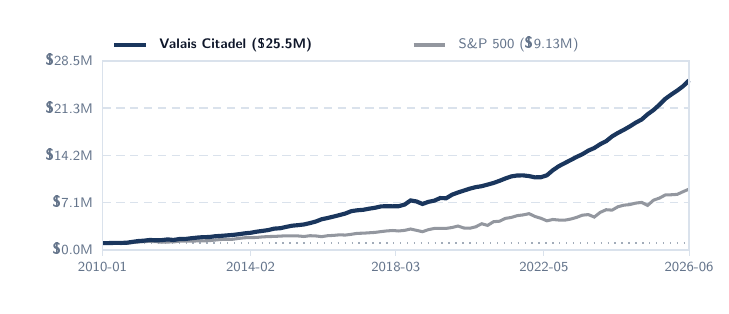
\begin{tikzpicture}[x=1cm, y=1cm]
    \useasboundingbox (-0.95,-0.46) rectangle (7.60,2.82);
    \draw[cardborder, densely dashed, line width=0.4pt] (0,0.000) -- (7.450,0.000);
\node[anchor=east, font=\sffamily\tiny, text=mutedtext, inner sep=1.5pt] at (-0.06,0.000) {\$0.0M};
\draw[cardborder, densely dashed, line width=0.4pt] (0,0.600) -- (7.450,0.600);
\node[anchor=east, font=\sffamily\tiny, text=mutedtext, inner sep=1.5pt] at (-0.06,0.600) {\$7.1M};
\draw[cardborder, densely dashed, line width=0.4pt] (0,1.200) -- (7.450,1.200);
\node[anchor=east, font=\sffamily\tiny, text=mutedtext, inner sep=1.5pt] at (-0.06,1.200) {\$14.2M};
\draw[cardborder, densely dashed, line width=0.4pt] (0,1.800) -- (7.450,1.800);
\node[anchor=east, font=\sffamily\tiny, text=mutedtext, inner sep=1.5pt] at (-0.06,1.800) {\$21.3M};
\draw[cardborder, densely dashed, line width=0.4pt] (0,2.400) -- (7.450,2.400);
\node[anchor=east, font=\sffamily\tiny, text=mutedtext, inner sep=1.5pt] at (-0.06,2.400) {\$28.5M};
\draw[mutedtext!60, dotted, line width=0.5pt] (0,0.084) -- (7.450,0.084);

    \fill[accent!10!white] (0.000,0.000) (0.000,0.084) (0.075,0.084) (0.151,0.087) (0.226,0.087) (0.301,0.088) (0.376,0.099) (0.452,0.110) (0.527,0.115) (0.602,0.124) (0.677,0.120) (0.753,0.122) (0.828,0.131) (0.903,0.124) (0.978,0.136) (1.054,0.137) (1.129,0.146) (1.204,0.154) (1.279,0.160) (1.355,0.161) (1.430,0.171) (1.505,0.176) (1.580,0.182) (1.656,0.188) (1.731,0.197) (1.806,0.208) (1.881,0.215) (1.957,0.229) (2.032,0.239) (2.107,0.250) (2.182,0.268) (2.258,0.273) (2.333,0.290) (2.408,0.305) (2.483,0.312) (2.559,0.321) (2.634,0.338) (2.709,0.358) (2.784,0.387) (2.860,0.403) (2.935,0.421) (3.010,0.440) (3.085,0.460) (3.161,0.490) (3.236,0.501) (3.311,0.507) (3.386,0.521) (3.462,0.533) (3.537,0.550) (3.612,0.553) (3.687,0.551) (3.763,0.553) (3.838,0.574) (3.913,0.626) (3.988,0.613) (4.064,0.581) (4.139,0.608) (4.214,0.623) (4.289,0.656) (4.365,0.654) (4.440,0.699) (4.515,0.727) (4.590,0.751) (4.666,0.776) (4.741,0.795) (4.816,0.807) (4.891,0.827) (4.967,0.848) (5.042,0.875) (5.117,0.905) (5.192,0.931) (5.268,0.943) (5.343,0.944) (5.418,0.935) (5.493,0.919) (5.569,0.921) (5.644,0.945) (5.719,1.009) (5.794,1.060) (5.870,1.100) (5.945,1.138) (6.020,1.178) (6.095,1.213) (6.171,1.259) (6.246,1.292) (6.321,1.340) (6.396,1.378) (6.472,1.439) (6.547,1.484) (6.622,1.523) (6.697,1.566) (6.773,1.614) (6.848,1.654) (6.923,1.720) (6.998,1.774) (7.074,1.842) (7.149,1.917) (7.224,1.971) (7.299,2.021) (7.375,2.078) (7.450,2.151) (7.450,0.000) -- cycle;
    \draw[primary!45, line width=1.1pt] plot coordinates {(0.000,0.084) (0.075,0.084) (0.151,0.090) (0.226,0.079) (0.301,0.080) (0.376,0.091) (0.452,0.097) (0.527,0.103) (0.602,0.106) (0.677,0.103) (0.753,0.095) (0.828,0.098) (0.903,0.099) (0.978,0.108) (1.054,0.111) (1.129,0.108) (1.204,0.112) (1.279,0.113) (1.355,0.115) (1.430,0.123) (1.505,0.130) (1.580,0.131) (1.656,0.133) (1.731,0.144) (1.806,0.152) (1.881,0.154) (1.957,0.156) (2.032,0.163) (2.107,0.167) (2.182,0.169) (2.258,0.173) (2.333,0.177) (2.408,0.176) (2.483,0.175) (2.559,0.168) (2.634,0.178) (2.709,0.175) (2.784,0.166) (2.860,0.178) (2.935,0.182) (3.010,0.189) (3.085,0.186) (3.161,0.196) (3.236,0.208) (3.311,0.210) (3.386,0.215) (3.462,0.220) (3.537,0.230) (3.612,0.239) (3.687,0.244) (3.763,0.238) (3.838,0.246) (3.913,0.263) (3.988,0.246) (4.064,0.229) (4.139,0.255) (4.214,0.270) (4.289,0.271) (4.365,0.271) (4.440,0.282) (4.515,0.301) (4.590,0.276) (4.666,0.273) (4.741,0.291) (4.816,0.330) (4.891,0.309) (4.967,0.356) (5.042,0.362) (5.117,0.398) (5.192,0.410) (5.268,0.433) (5.343,0.442) (5.418,0.458) (5.493,0.422) (5.569,0.399) (5.644,0.367) (5.719,0.384) (5.794,0.377) (5.870,0.375) (5.945,0.389) (6.020,0.410) (6.095,0.439) (6.171,0.446) (6.246,0.415) (6.321,0.474) (6.396,0.508) (6.472,0.503) (6.547,0.546) (6.622,0.566) (6.697,0.573) (6.773,0.592) (6.848,0.601) (6.923,0.563) (6.998,0.629) (7.074,0.656) (7.149,0.696) (7.224,0.698) (7.299,0.703) (7.375,0.738) (7.450,0.770)};
    \draw[accent, line width=1.5pt] plot coordinates {(0.000,0.084) (0.075,0.084) (0.151,0.087) (0.226,0.087) (0.301,0.088) (0.376,0.099) (0.452,0.110) (0.527,0.115) (0.602,0.124) (0.677,0.120) (0.753,0.122) (0.828,0.131) (0.903,0.124) (0.978,0.136) (1.054,0.137) (1.129,0.146) (1.204,0.154) (1.279,0.160) (1.355,0.161) (1.430,0.171) (1.505,0.176) (1.580,0.182) (1.656,0.188) (1.731,0.197) (1.806,0.208) (1.881,0.215) (1.957,0.229) (2.032,0.239) (2.107,0.250) (2.182,0.268) (2.258,0.273) (2.333,0.290) (2.408,0.305) (2.483,0.312) (2.559,0.321) (2.634,0.338) (2.709,0.358) (2.784,0.387) (2.860,0.403) (2.935,0.421) (3.010,0.440) (3.085,0.460) (3.161,0.490) (3.236,0.501) (3.311,0.507) (3.386,0.521) (3.462,0.533) (3.537,0.550) (3.612,0.553) (3.687,0.551) (3.763,0.553) (3.838,0.574) (3.913,0.626) (3.988,0.613) (4.064,0.581) (4.139,0.608) (4.214,0.623) (4.289,0.656) (4.365,0.654) (4.440,0.699) (4.515,0.727) (4.590,0.751) (4.666,0.776) (4.741,0.795) (4.816,0.807) (4.891,0.827) (4.967,0.848) (5.042,0.875) (5.117,0.905) (5.192,0.931) (5.268,0.943) (5.343,0.944) (5.418,0.935) (5.493,0.919) (5.569,0.921) (5.644,0.945) (5.719,1.009) (5.794,1.060) (5.870,1.100) (5.945,1.138) (6.020,1.178) (6.095,1.213) (6.171,1.259) (6.246,1.292) (6.321,1.340) (6.396,1.378) (6.472,1.439) (6.547,1.484) (6.622,1.523) (6.697,1.566) (6.773,1.614) (6.848,1.654) (6.923,1.720) (6.998,1.774) (7.074,1.842) (7.149,1.917) (7.224,1.971) (7.299,2.021) (7.375,2.078) (7.450,2.151)};
    \draw[cardborder, line width=0.6pt] (0,0) rectangle (7.450,2.400);
    \draw[cardborder, line width=0.4pt] (0.000,0) -- (0.000,-0.08);
\node[anchor=north, font=\sffamily\tiny, text=mutedtext, inner sep=1.5pt] at (0.000,-0.10) {2010-01};
\draw[cardborder, line width=0.4pt] (1.881,0) -- (1.881,-0.08);
\node[anchor=north, font=\sffamily\tiny, text=mutedtext, inner sep=1.5pt] at (1.881,-0.10) {2014-02};
\draw[cardborder, line width=0.4pt] (3.725,0) -- (3.725,-0.08);
\node[anchor=north, font=\sffamily\tiny, text=mutedtext, inner sep=1.5pt] at (3.725,-0.10) {2018-03};
\draw[cardborder, line width=0.4pt] (5.606,0) -- (5.606,-0.08);
\node[anchor=north, font=\sffamily\tiny, text=mutedtext, inner sep=1.5pt] at (5.606,-0.10) {2022-05};
\draw[cardborder, line width=0.4pt] (7.450,0) -- (7.450,-0.08);
\node[anchor=north, font=\sffamily\tiny, text=mutedtext, inner sep=1.5pt] at (7.450,-0.10) {2026-06};

    % Legend
    \draw[accent, line width=1.6pt] (0.15,2.600) -- (0.55,2.600);
    \node[anchor=west, font=\sffamily\tiny\bfseries, text=primary] at (0.60,2.600) {Valais Citadel (\$25.5M)};
    \draw[primary!45, line width=1.2pt] (3.95,2.600) -- (4.35,2.600);
    \node[anchor=west, font=\sffamily\tiny, text=mutedtext] at (4.40,2.600) {S\&P 500 (\$9.13M)};
\end{tikzpicture}
\end{tcolorbox}\hfill
\begin{tcolorbox}[nobeforeafter, box align=top, width=0.492\textwidth, colback=white, colframe=primary, title=\textbf{\small\strut Worst 20\% S\&P 500 Months}, fonttitle=\sffamily\bfseries\small, arc=5pt, boxrule=0.9pt, toptitle=3.5pt, bottomtitle=3.5pt, left=4pt, right=4pt, top=3pt, bottom=2pt, colbacktitle=primary, halign title=center]
\centering
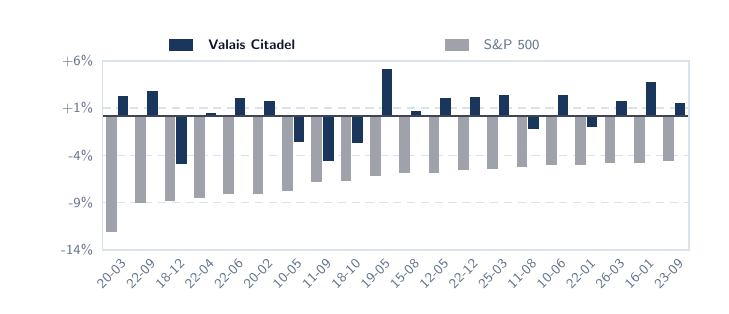
\begin{tikzpicture}[x=1cm, y=1cm]
    \useasboundingbox (-0.95,-0.46) rectangle (7.60,2.82);
    \draw[cardborder, densely dashed, line width=0.4pt] (0,0.000) -- (7.450,0.000);
\node[anchor=east, font=\sffamily\tiny, text=mutedtext, inner sep=1.5pt] at (-0.06,0.000) {-14\%};
\draw[cardborder, densely dashed, line width=0.4pt] (0,0.600) -- (7.450,0.600);
\node[anchor=east, font=\sffamily\tiny, text=mutedtext, inner sep=1.5pt] at (-0.06,0.600) {-9\%};
\draw[cardborder, densely dashed, line width=0.4pt] (0,1.200) -- (7.450,1.200);
\node[anchor=east, font=\sffamily\tiny, text=mutedtext, inner sep=1.5pt] at (-0.06,1.200) {-4\%};
\draw[cardborder, densely dashed, line width=0.4pt] (0,1.800) -- (7.450,1.800);
\node[anchor=east, font=\sffamily\tiny, text=mutedtext, inner sep=1.5pt] at (-0.06,1.800) {+1\%};
\draw[cardborder, densely dashed, line width=0.4pt] (0,2.400) -- (7.450,2.400);
\node[anchor=east, font=\sffamily\tiny, text=mutedtext, inner sep=1.5pt] at (-0.06,2.400) {+6\%};

    \fill[primary!40] (0.046,0.221) rectangle (0.180,1.695);
\fill[accent] (0.192,1.695) rectangle (0.326,1.949);
\node[rotate=45, anchor=north east, font=\sffamily\fontsize{4.6}{5.6}\selectfont, text=mutedtext, inner sep=0.8pt] at (0.226,-0.06) {20-03};
\fill[primary!40] (0.419,0.596) rectangle (0.553,1.695);
\fill[accent] (0.565,1.695) rectangle (0.699,2.022);
\node[rotate=45, anchor=north east, font=\sffamily\fontsize{4.6}{5.6}\selectfont, text=mutedtext, inner sep=0.8pt] at (0.599,-0.06) {22-09};
\fill[primary!40] (0.791,0.617) rectangle (0.925,1.695);
\fill[accent] (0.937,1.090) rectangle (1.071,1.695);
\node[rotate=45, anchor=north east, font=\sffamily\fontsize{4.6}{5.6}\selectfont, text=mutedtext, inner sep=0.8pt] at (0.971,-0.06) {18-12};
\fill[primary!40] (1.164,0.654) rectangle (1.298,1.695);
\fill[accent] (1.310,1.695) rectangle (1.444,1.739);
\node[rotate=45, anchor=north east, font=\sffamily\fontsize{4.6}{5.6}\selectfont, text=mutedtext, inner sep=0.8pt] at (1.344,-0.06) {22-04};
\fill[primary!40] (1.536,0.710) rectangle (1.670,1.695);
\fill[accent] (1.682,1.695) rectangle (1.816,1.926);
\node[rotate=45, anchor=north east, font=\sffamily\fontsize{4.6}{5.6}\selectfont, text=mutedtext, inner sep=0.8pt] at (1.716,-0.06) {22-06};
\fill[primary!40] (1.909,0.713) rectangle (2.043,1.695);
\fill[accent] (2.055,1.695) rectangle (2.189,1.887);
\node[rotate=45, anchor=north east, font=\sffamily\fontsize{4.6}{5.6}\selectfont, text=mutedtext, inner sep=0.8pt] at (2.089,-0.06) {20-02};
\fill[primary!40] (2.281,0.742) rectangle (2.415,1.695);
\fill[accent] (2.427,1.370) rectangle (2.561,1.695);
\node[rotate=45, anchor=north east, font=\sffamily\fontsize{4.6}{5.6}\selectfont, text=mutedtext, inner sep=0.8pt] at (2.461,-0.06) {10-05};
\fill[primary!40] (2.654,0.856) rectangle (2.788,1.695);
\fill[accent] (2.800,1.124) rectangle (2.934,1.695);
\node[rotate=45, anchor=north east, font=\sffamily\fontsize{4.6}{5.6}\selectfont, text=mutedtext, inner sep=0.8pt] at (2.834,-0.06) {11-09};
\fill[primary!40] (3.026,0.879) rectangle (3.160,1.695);
\fill[accent] (3.172,1.361) rectangle (3.306,1.695);
\node[rotate=45, anchor=north east, font=\sffamily\fontsize{4.6}{5.6}\selectfont, text=mutedtext, inner sep=0.8pt] at (3.206,-0.06) {18-10};
\fill[primary!40] (3.399,0.936) rectangle (3.533,1.695);
\fill[accent] (3.545,1.695) rectangle (3.679,2.292);
\node[rotate=45, anchor=north east, font=\sffamily\fontsize{4.6}{5.6}\selectfont, text=mutedtext, inner sep=0.8pt] at (3.579,-0.06) {19-05};
\fill[primary!40] (3.771,0.975) rectangle (3.905,1.695);
\fill[accent] (3.917,1.695) rectangle (4.051,1.766);
\node[rotate=45, anchor=north east, font=\sffamily\fontsize{4.6}{5.6}\selectfont, text=mutedtext, inner sep=0.8pt] at (3.951,-0.06) {15-08};
\fill[primary!40] (4.144,0.978) rectangle (4.278,1.695);
\fill[accent] (4.290,1.695) rectangle (4.424,1.923);
\node[rotate=45, anchor=north east, font=\sffamily\fontsize{4.6}{5.6}\selectfont, text=mutedtext, inner sep=0.8pt] at (4.324,-0.06) {12-05};
\fill[primary!40] (4.516,1.007) rectangle (4.650,1.695);
\fill[accent] (4.662,1.695) rectangle (4.796,1.940);
\node[rotate=45, anchor=north east, font=\sffamily\fontsize{4.6}{5.6}\selectfont, text=mutedtext, inner sep=0.8pt] at (4.696,-0.06) {22-12};
\fill[primary!40] (4.889,1.022) rectangle (5.023,1.695);
\fill[accent] (5.035,1.695) rectangle (5.169,1.970);
\node[rotate=45, anchor=north east, font=\sffamily\fontsize{4.6}{5.6}\selectfont, text=mutedtext, inner sep=0.8pt] at (5.069,-0.06) {25-03};
\fill[primary!40] (5.261,1.047) rectangle (5.395,1.695);
\fill[accent] (5.407,1.528) rectangle (5.541,1.695);
\node[rotate=45, anchor=north east, font=\sffamily\fontsize{4.6}{5.6}\selectfont, text=mutedtext, inner sep=0.8pt] at (5.441,-0.06) {11-08};
\fill[primary!40] (5.634,1.070) rectangle (5.768,1.695);
\fill[accent] (5.780,1.695) rectangle (5.914,1.963);
\node[rotate=45, anchor=north east, font=\sffamily\fontsize{4.6}{5.6}\selectfont, text=mutedtext, inner sep=0.8pt] at (5.814,-0.06) {10-06};
\fill[primary!40] (6.006,1.077) rectangle (6.140,1.695);
\fill[accent] (6.152,1.557) rectangle (6.286,1.695);
\node[rotate=45, anchor=north east, font=\sffamily\fontsize{4.6}{5.6}\selectfont, text=mutedtext, inner sep=0.8pt] at (6.186,-0.06) {22-01};
\fill[primary!40] (6.379,1.101) rectangle (6.513,1.695);
\fill[accent] (6.525,1.695) rectangle (6.659,1.886);
\node[rotate=45, anchor=north east, font=\sffamily\fontsize{4.6}{5.6}\selectfont, text=mutedtext, inner sep=0.8pt] at (6.559,-0.06) {26-03};
\fill[primary!40] (6.751,1.103) rectangle (6.885,1.695);
\fill[accent] (6.897,1.695) rectangle (7.031,2.124);
\node[rotate=45, anchor=north east, font=\sffamily\fontsize{4.6}{5.6}\selectfont, text=mutedtext, inner sep=0.8pt] at (6.931,-0.06) {16-01};
\fill[primary!40] (7.124,1.126) rectangle (7.258,1.695);
\fill[accent] (7.270,1.695) rectangle (7.404,1.858);
\node[rotate=45, anchor=north east, font=\sffamily\fontsize{4.6}{5.6}\selectfont, text=mutedtext, inner sep=0.8pt] at (7.304,-0.06) {23-09};
\draw[primary!80, line width=0.55pt] (0,1.695) -- (7.450,1.695);

    \draw[cardborder, line width=0.6pt] (0,0) rectangle (7.450,2.400);
    % Legend
    \fill[accent] (0.85,2.530) rectangle (1.15,2.670);
    \node[anchor=west, font=\sffamily\tiny\bfseries, text=primary] at (1.22,2.600) {Valais Citadel};
    \fill[primary!40] (4.35,2.530) rectangle (4.65,2.670);
    \node[anchor=west, font=\sffamily\tiny, text=mutedtext] at (4.72,2.600) {S\&P 500};
\end{tikzpicture}
\end{tcolorbox}


\vspace{0.25em}

% --- SECTION 4: MONTHLY RETURN MATRIX (NO BLACK HORIZONTAL RULES) ---
\begin{tcolorbox}[colback=white, colframe=primary, title=\textbf{\small\strut Historical Monthly \& Yearly Net Return Matrix (\%)}, fonttitle=\sffamily\bfseries\small, arc=5pt, boxrule=0.9pt, toptitle=3.5pt, bottomtitle=3.5pt, left=3pt, right=3pt, top=2pt, bottom=2pt, colbacktitle=primary, halign title=center]
\renewcommand{\arraystretch}{1.14}
\scriptsize
\begin{tabularx}{\textwidth}{l *{12}{>{\centering\arraybackslash}X} >{\centering\arraybackslash}p{1.15cm}}
\rowcolor{primary!8!white}
\textbf{\textcolor{primary}{Year}} & \textbf{\textcolor{primary}{Jan}} & \textbf{\textcolor{primary}{Feb}} & \textbf{\textcolor{primary}{Mar}} & \textbf{\textcolor{primary}{Apr}} & \textbf{\textcolor{primary}{May}} & \textbf{\textcolor{primary}{Jun}} & \textbf{\textcolor{primary}{Jul}} & \textbf{\textcolor{primary}{Aug}} & \textbf{\textcolor{primary}{Sep}} & \textbf{\textcolor{primary}{Oct}} & \textbf{\textcolor{primary}{Nov}} & \textbf{\textcolor{primary}{Dec}} & \textbf{\textcolor{primary}{Yearly}} \\
\textbf{2010} & \cellcolor{negred!8!white}-1.1\% & \cellcolor{posgreen!7!white}1.0\% & \cellcolor{posgreen!16!white}2.2\% & \cellcolor{posgreen!11!white}1.5\% & \cellcolor{negred!20!white}-2.7\% & \cellcolor{posgreen!16!white}2.2\% & \cellcolor{negred!25!white}-3.5\% & \cellcolor{posgreen!33!white}4.5\% & \cellcolor{posgreen!75!white}10.7\% & \cellcolor{posgreen!18!white}2.4\% & \cellcolor{posgreen!38!white}5.2\% & \cellcolor{posgreen!39!white}5.3\% & \cellcolor{posgreen!75!white}\textbf{30.5\%} \\
\textbf{2011} & \cellcolor{negred!22!white}-3.1\% & \cellcolor{posgreen!58!white}7.8\% & \cellcolor{posgreen!11!white}1.5\% & \cellcolor{posgreen!46!white}6.2\% & \cellcolor{negred!16!white}-2.1\% & \cellcolor{negred!9!white}-1.3\% & \cellcolor{posgreen!23!white}3.2\% & \cellcolor{negred!10!white}-1.4\% & \cellcolor{negred!35!white}-4.8\% & \cellcolor{posgreen!75!white}12.6\% & \cellcolor{negred!10!white}-1.4\% & \cellcolor{negred!29!white}-4.0\% & \cellcolor{posgreen!39!white}\textbf{12.3\%} \\
\textbf{2012} & \cellcolor{posgreen!53!white}7.1\% & \cellcolor{posgreen!20!white}2.7\% & \cellcolor{posgreen!4!white}0.1\% & \cellcolor{posgreen!4!white}0.5\% & \cellcolor{posgreen!14!white}1.9\% & \cellcolor{posgreen!37!white}5.0\% & \cellcolor{posgreen!13!white}1.8\% & \cellcolor{posgreen!28!white}3.7\% & \cellcolor{posgreen!25!white}3.4\% & \cellcolor{posgreen!4!white}0.3\% & \cellcolor{posgreen!4!white}0.5\% & \cellcolor{posgreen!4!white}0.2\% & \cellcolor{posgreen!75!white}\textbf{30.6\%} \\
\textbf{2013} & \cellcolor{posgreen!18!white}2.5\% & \cellcolor{posgreen!25!white}3.4\% & \cellcolor{posgreen!7!white}0.9\% & \cellcolor{posgreen!14!white}1.9\% & \cellcolor{posgreen!11!white}1.5\% & \cellcolor{posgreen!15!white}2.1\% & \cellcolor{posgreen!4!white}0.2\% & \cellcolor{posgreen!21!white}2.9\% & \cellcolor{posgreen!18!white}2.5\% & \cellcolor{posgreen!17!white}2.3\% & \cellcolor{posgreen!18!white}2.5\% & \cellcolor{posgreen!23!white}3.1\% & \cellcolor{posgreen!75!white}\textbf{29.0\%} \\
\textbf{2014} & \cellcolor{posgreen!10!white}1.4\% & \cellcolor{posgreen!13!white}1.7\% & \cellcolor{posgreen!30!white}4.0\% & \cellcolor{posgreen!18!white}2.4\% & \cellcolor{posgreen!23!white}3.1\% & \cellcolor{posgreen!11!white}1.5\% & \cellcolor{posgreen!16!white}2.2\% & \cellcolor{posgreen!16!white}2.2\% & \cellcolor{posgreen!21!white}2.8\% & \cellcolor{posgreen!33!white}4.5\% & \cellcolor{posgreen!6!white}0.9\% & \cellcolor{posgreen!5!white}0.8\% & \cellcolor{posgreen!75!white}\textbf{31.2\%} \\
\textbf{2015} & \cellcolor{posgreen!35!white}4.7\% & \cellcolor{posgreen!12!white}1.6\% & \cellcolor{posgreen!26!white}3.6\% & \cellcolor{posgreen!11!white}1.5\% & \cellcolor{posgreen!12!white}1.7\% & \cellcolor{posgreen!4!white}0.6\% & \cellcolor{posgreen!17!white}2.4\% & \cellcolor{posgreen!4!white}0.6\% & \cellcolor{posgreen!13!white}1.8\% & \cellcolor{posgreen!24!white}3.2\% & \cellcolor{posgreen!25!white}3.3\% & \cellcolor{posgreen!20!white}2.7\% & \cellcolor{posgreen!75!white}\textbf{31.3\%} \\
\textbf{2016} & \cellcolor{posgreen!27!white}3.6\% & \cellcolor{posgreen!32!white}4.3\% & \cellcolor{posgreen!13!white}1.9\% & \cellcolor{posgreen!17!white}2.3\% & \cellcolor{posgreen!12!white}1.7\% & \cellcolor{posgreen!20!white}2.7\% & \cellcolor{posgreen!16!white}2.2\% & \cellcolor{posgreen!16!white}2.3\% & \cellcolor{posgreen!21!white}2.8\% & \cellcolor{posgreen!12!white}1.7\% & \cellcolor{posgreen!29!white}3.9\% & \cellcolor{posgreen!18!white}2.5\% & \cellcolor{posgreen!75!white}\textbf{36.8\%} \\
\textbf{2017} & \cellcolor{posgreen!10!white}1.3\% & \cellcolor{posgreen!6!white}0.9\% & \cellcolor{posgreen!7!white}1.0\% & \cellcolor{posgreen!4!white}0.2\% & \cellcolor{posgreen!18!white}2.4\% & \cellcolor{posgreen!4!white}0.2\% & \cellcolor{posgreen!19!white}2.6\% & \cellcolor{negred!4!white}-0.2\% & \cellcolor{posgreen!6!white}0.8\% & \cellcolor{posgreen!18!white}2.5\% & \cellcolor{negred!4!white}-0.4\% & \cellcolor{posgreen!7!white}1.0\% & \cellcolor{posgreen!41!white}\textbf{12.9\%} \\
\textbf{2018} & \cellcolor{posgreen!10!white}1.4\% & \cellcolor{negred!13!white}-1.8\% & \cellcolor{posgreen!4!white}0.5\% & \cellcolor{negred!4!white}-0.1\% & \cellcolor{posgreen!21!white}2.9\% & \cellcolor{posgreen!6!white}0.8\% & \cellcolor{posgreen!29!white}4.0\% & \cellcolor{posgreen!37!white}5.0\% & \cellcolor{posgreen!4!white}0.7\% & \cellcolor{negred!20!white}-2.8\% & \cellcolor{negred!4!white}-0.0\% & \cellcolor{negred!38!white}-5.1\% & \cellcolor{posgreen!16!white}\textbf{5.0\%} \\
\textbf{2019} & \cellcolor{posgreen!30!white}4.1\% & \cellcolor{posgreen!4!white}0.6\% & \cellcolor{posgreen!4!white}0.7\% & \cellcolor{posgreen!12!white}1.7\% & \cellcolor{posgreen!37!white}5.0\% & \cellcolor{posgreen!4!white}0.4\% & \cellcolor{negred!4!white}-0.2\% & \cellcolor{negred!4!white}-0.2\% & \cellcolor{posgreen!21!white}2.8\% & \cellcolor{posgreen!29!white}4.0\% & \cellcolor{negred!8!white}-1.2\% & \cellcolor{posgreen!39!white}5.2\% & \cellcolor{posgreen!75!white}\textbf{25.0\%} \\
\textbf{2020} & \cellcolor{posgreen!12!white}1.7\% & \cellcolor{posgreen!12!white}1.6\% & \cellcolor{posgreen!15!white}2.1\% & \cellcolor{posgreen!9!white}1.2\% & \cellcolor{posgreen!9!white}1.3\% & \cellcolor{posgreen!9!white}1.2\% & \cellcolor{posgreen!6!white}0.9\% & \cellcolor{posgreen!4!white}0.6\% & \cellcolor{posgreen!10!white}1.4\% & \cellcolor{posgreen!8!white}1.1\% & \cellcolor{posgreen!8!white}1.1\% & \cellcolor{posgreen!11!white}1.5\% & \cellcolor{posgreen!53!white}\textbf{16.7\%} \\
\textbf{2021} & \cellcolor{posgreen!9!white}1.3\% & \cellcolor{posgreen!14!white}1.9\% & \cellcolor{posgreen!14!white}1.9\% & \cellcolor{posgreen!10!white}1.4\% & \cellcolor{posgreen!14!white}1.9\% & \cellcolor{posgreen!7!white}1.0\% & \cellcolor{posgreen!8!white}1.1\% & \cellcolor{posgreen!4!white}0.1\% & \cellcolor{negred!7!white}-0.9\% & \cellcolor{posgreen!7!white}1.0\% & \cellcolor{negred!4!white}-0.4\% & \cellcolor{negred!4!white}-0.5\% & \cellcolor{posgreen!32!white}\textbf{10.3\%} \\
\textbf{2022} & \cellcolor{negred!8!white}-1.1\% & \cellcolor{negred!4!white}-0.6\% & \cellcolor{negred!4!white}-0.2\% & \cellcolor{posgreen!4!white}0.4\% & \cellcolor{posgreen!4!white}0.7\% & \cellcolor{posgreen!14!white}1.9\% & \cellcolor{posgreen!29!white}3.9\% & \cellcolor{posgreen!21!white}2.8\% & \cellcolor{posgreen!20!white}2.7\% & \cellcolor{posgreen!16!white}2.2\% & \cellcolor{posgreen!12!white}1.7\% & \cellcolor{posgreen!15!white}2.1\% & \cellcolor{posgreen!56!white}\textbf{17.6\%} \\
\textbf{2023} & \cellcolor{posgreen!12!white}1.7\% & \cellcolor{posgreen!12!white}1.7\% & \cellcolor{posgreen!14!white}1.9\% & \cellcolor{posgreen!12!white}1.6\% & \cellcolor{posgreen!15!white}2.0\% & \cellcolor{posgreen!6!white}0.9\% & \cellcolor{posgreen!15!white}2.1\% & \cellcolor{posgreen!12!white}1.7\% & \cellcolor{posgreen!10!white}1.4\% & \cellcolor{posgreen!9!white}1.2\% & \cellcolor{posgreen!10!white}1.4\% & \cellcolor{posgreen!17!white}2.3\% & \cellcolor{posgreen!69!white}\textbf{21.8\%} \\
\textbf{2024} & \cellcolor{posgreen!13!white}1.8\% & \cellcolor{posgreen!7!white}0.9\% & \cellcolor{posgreen!16!white}2.3\% & \cellcolor{posgreen!16!white}2.2\% & \cellcolor{posgreen!14!white}2.0\% & \cellcolor{posgreen!8!white}1.1\% & \cellcolor{posgreen!10!white}1.3\% & \cellcolor{posgreen!9!white}1.3\% & \cellcolor{posgreen!8!white}1.1\% & \cellcolor{posgreen!12!white}1.7\% & \cellcolor{posgreen!12!white}1.7\% & \cellcolor{posgreen!9!white}1.3\% & \cellcolor{posgreen!65!white}\textbf{20.4\%} \\
\textbf{2025} & \cellcolor{posgreen!11!white}1.5\% & \cellcolor{posgreen!6!white}0.9\% & \cellcolor{posgreen!17!white}2.3\% & \cellcolor{posgreen!12!white}1.7\% & \cellcolor{posgreen!11!white}1.5\% & \cellcolor{posgreen!11!white}1.6\% & \cellcolor{posgreen!19!white}2.5\% & \cellcolor{posgreen!9!white}1.3\% & \cellcolor{posgreen!14!white}1.9\% & \cellcolor{posgreen!15!white}2.1\% & \cellcolor{posgreen!9!white}1.2\% & \cellcolor{posgreen!11!white}1.6\% & \cellcolor{posgreen!70!white}\textbf{22.2\%} \\
\textbf{2026} & \cellcolor{posgreen!10!white}1.4\% & \cellcolor{posgreen!8!white}1.1\% & \cellcolor{posgreen!12!white}1.6\% & \cellcolor{posgreen!9!white}1.2\% & \cellcolor{posgreen!17!white}2.4\% & \cellcolor{posgreen!8!white}1.1\% & \textcolor{gray!60}{-} & \textcolor{gray!60}{-} & \textcolor{gray!60}{-} & \textcolor{gray!60}{-} & \textcolor{gray!60}{-} & \textcolor{gray!60}{-} & \cellcolor{posgreen!29!white}\textbf{9.1\%} \\
\end{tabularx}
\end{tcolorbox}
\vspace{0.25em}

% --- SECTION 5: FUND TERMS & COMMERCIAL OVERVIEW BOX (BOTTOM OF PAGE 1) ---
\begin{tcolorbox}[colback=white, colframe=primary, title=\textbf{\small\strut Fund Terms \& Commercial Overview}, fonttitle=\sffamily\bfseries\small, arc=5pt, boxrule=0.9pt, toptitle=3.5pt, bottomtitle=3.5pt, left=4pt, right=4pt, top=2.5pt, bottom=2.5pt, colbacktitle=primary, halign title=center]
\renewcommand{\arraystretch}{1.38}
\setlength{\tabcolsep}{6pt}
\scriptsize
\begin{tabularx}{\textwidth}{X !{\color{cardborder}\vrule width 0.6pt} X !{\color{cardborder}\vrule width 0.6pt} X !{\color{cardborder}\vrule width 0.6pt} X}
\textbf{\textcolor{mutedtext}{\strut Vehicle:}}\hfill \textbf{\textcolor{primary}{\strut Commingled Fund}} & \textbf{\textcolor{mutedtext}{\strut Return Basis:}}\hfill \textbf{\textcolor{primary}{\strut Net of Fees}} & \textbf{\textcolor{mutedtext}{\strut Fee Structure:}}\hfill \textbf{\textcolor{primary}{\strut 2\% Mgmt / 20\% Perf}} & \textbf{\textcolor{mutedtext}{\strut Liquidity:}}\hfill \textbf{\textcolor{primary}{\strut Quarter Liquidity}} \\
\rowcolor{cardbg} \textbf{\textcolor{mutedtext}{\strut Lock-Up Period:}}\hfill \textbf{\textcolor{primary}{\strut No Lockup}} & \textbf{\textcolor{mutedtext}{\strut Min. Investment:}}\hfill \textbf{\textcolor{primary}{\strut 1M USD}} & \textbf{\textcolor{mutedtext}{\strut Current AUM:}}\hfill \textbf{\textcolor{primary}{\strut 250M}} & \textbf{\textcolor{mutedtext}{\strut Domicile:}}\hfill \textbf{\textcolor{primary}{\strut Cayman Islands}} \\
\end{tabularx}
\end{tcolorbox}

\vfill

% --- PAGE 1 FOOTER ---
\noindent{\color{cardborder}\rule{\textwidth}{0.6pt}}\\[2pt]
\noindent
\begin{minipage}[c]{0.74\textwidth}
    {\tiny \textcolor{mutedtext}{\textbf{Ath\'en\'ee Investment} $\vert$ Quai des Bergues 23, 1201 Geneva, Switzerland $\vert$ \href{mailto:arthur.dhonneur@athenee-investment.com}{arthur.dhonneur@athenee-investment.com}}\\[1pt]
    \tiny \textcolor{mutedtext}{\textit{Capital Introduction \& Third-Party Marketing Memorandum. Strictly for Institutional \& Qualified Investors. Please see Page 2 for Risk \& Legal Disclosures.}}}
\end{minipage}%
\hfill
\begin{minipage}[c]{0.24\textwidth}
    \raggedleft
    {\tiny \bfseries \textcolor{primary}{Page 1 of 2}}
\end{minipage}

\clearpage

%%%%%%%%%%%%%%%%%%%%%%%%%%%%%%%%%%%%%%%%%%%%%%%%%%%%%%%%%%%%%%%%%%%%%%%%%%%%%%%
%% PAGE 2: LEGAL DISCLAIMER (TOP) + QUANTITATIVE METHODOLOGY & APPENDIX
%%%%%%%%%%%%%%%%%%%%%%%%%%%%%%%%%%%%%%%%%%%%%%%%%%%%%%%%%%%%%%%%%%%%%%%%%%%%%%%

% --- PAGE 2 HEADER ---
\noindent
\begin{minipage}[c]{0.68\textwidth}
    {\Large \bfseries \textcolor{primary}{Risk Disclosures, Legal Notice \& Quantitative Appendix}}\\[2pt]
    {\footnotesize \bfseries \textcolor{accent}{Fund Reference: Valais Citadel (ATH-804) (Jan 2010 - Jun 2026 (198 Months / 16.5 Years))}}
\end{minipage}%
\hfill
\begin{minipage}[c]{0.30\textwidth}
    \raggedleft
    
\includegraphics[height=1.0cm, keepaspectratio]{athenee_logo.png}\\[2pt]
    {\tiny \bfseries \textcolor{goldaccent}{CAPITAL INTRODUCTION \& THIRD-PARTY MARKETING}}
\end{minipage}

\vspace{0.3em}
\noindent{\color{goldaccent}\rule{\textwidth}{1.2pt}}
\vspace{0.4em}

% --- PART I (TOP OF PAGE 2): CAPITAL INTRODUCTION & RISK DISCLAIMER ---
\begin{tcolorbox}[colback=white, colframe=accent, title=\textbf{\small\strut Important Legal Disclaimer, Risk Disclosures \& Capital Introduction Notice}, fonttitle=\sffamily\bfseries\small, arc=5pt, boxrule=0.9pt, toptitle=4.5pt, bottomtitle=4.5pt, left=8pt, right=8pt, top=4.5pt, bottom=4.5pt, colbacktitle=accent]
\scriptsize
\textcolor{primary}{
\textbf{1. Role of Ath\'en\'ee Investment — Capital Introduction Services Only (No Investment Advice):}\\[1.5pt]
This document has been prepared by \textbf{Ath\'en\'ee Investment} solely for informational and discussion purposes as part of its institutional \textbf{Capital Introduction and Third-Party Marketing} activities. \textbf{This document does not constitute investment advice, financial advisory services, a personal recommendation, or an offer to sell or a solicitation of an offer to buy} any shares, units, or interests in any investment fund or financial instrument. Prospective investors must conduct their own independent due diligence and consult their own professional legal, regulatory, tax, and financial advisors before making any investment decision.\\[4.5pt]
\textbf{2. No Warranty of Data Accuracy or Completeness (Third-Party Manager Data):}\\[1.5pt]
All historical performance figures, return series, and strategy descriptions presented herein are derived from information provided directly by the respective third-party hedge fund managers or external data providers. While Ath\'en\'ee Investment has compiled and analyzed these quantitative metrics in good faith, \textbf{Ath\'en\'ee Investment has not independently audited or verified the underlying data and cannot guarantee—and makes no representation or warranty, express or implied, regarding—the accuracy, completeness, reliability, or timeliness} of any information contained in this document. Any errors, omissions, or subsequent restatements by the underlying fund manager are the sole responsibility of such manager.\\[4.5pt]
\textbf{3. Key Risk Factors of Alternative \& Hedge Fund Strategies:}\\[1.5pt]
Investing in alternative investment funds and hedge funds involves a \textbf{high degree of risk} and is suitable only for sophisticated investors capable of bearing the loss of their entire investment. Material risks include, without limitation:
\begin{itemize}[leftmargin=1.3em, itemsep=1pt, topsep=1pt]
    \item \textbf{Market, Leverage \& Derivative Risk:} Underlying funds may employ substantial leverage, short-selling, options, futures, swaps, and other derivative instruments, which can amplify both gains and losses and cause rapid capital erosion during extreme market dislocations.
    \item \textbf{Illiquidity \& Lock-Up Risk:} Hedge fund interests are typically not listed on any regulated exchange and are subject to redemption gates, notice periods, lock-ups, and side-pocket arrangements.
    \item \textbf{Model, Regime Shift \& Tail-Correlation Risk:} Quantitative and systematic strategies rely on mathematical models and historical statistical relationships (such as low equity beta or negative downside capture) that may break down or experience sudden correlation spikes during systemic liquidity crises.
    \item \textbf{Operational, Counterparty \& Valuation Risk:} Strategies trading in over-the-counter (OTC) derivatives, digital assets, distressed debt, or emerging markets face heightened counterparty default, custody, regulatory, and mark-to-model valuation risks.
\end{itemize}
\vspace{2.5pt}
\textbf{4. Past Performance \& Quantitative Limitations:}\\[1.5pt]
\textbf{Past performance is not indicative of, nor a guarantee of, future results.} The value of investments and the income derived from them may go down as well as up. Simulated, bootstrap, or regression-based indicators (including Alpha, Beta, Sharpe Ratio, Sortino Ratio, and Capture Ratios) are backward-looking statistical estimates and do not represent a promise or forecast of future risk-adjusted returns.\\[4.5pt]
\textbf{5. Qualified Investors Only \& Confidentiality:}\\[1.5pt]
This document is strictly confidential and is directed exclusively at \textbf{Institutional, Professional, and Qualified Investors} (including Qualified Investors within the meaning of the Swiss Collective Investment Schemes Act (CISA) and Financial Services Act (FinSA)). It may not be copied, reproduced, distributed, or disclosed to any third party, nor distributed in any jurisdiction where such distribution would be unlawful.
}
\end{tcolorbox}

\vspace{0.45em}

% --- PART II: EXTENDED SINGLE-FUND QUANTITATIVE DIAGNOSTICS ---
\begin{tcolorbox}[colback=white, colframe=primary, title=\textbf{\small\strut Appendix A: Extended Statistical, Bootstrap \& Factor Diagnostics}, fonttitle=\sffamily\bfseries\small, arc=5pt, boxrule=0.8pt, toptitle=4pt, bottomtitle=4pt, left=6pt, right=6pt, top=3.5pt, bottom=3.5pt, colbacktitle=primary]
\renewcommand{\arraystretch}{1.22}
\scriptsize
\begin{tabularx}{\textwidth}{l X r}
\toprule
\textbf{\textcolor{primary}{Diagnostic Family}} & \textbf{\textcolor{primary}{Methodology / Statistical Specification}} & \textbf{\textcolor{primary}{Empirical Value}} \\
\midrule
\textbf{Pearson Correlation CI} & 95\% Confidence Interval (IID Bootstrap vs. Moving Block $B=3$, 1,000 iters) & Std: [0.09, 0.43] $\vert$ Blk: [0.09, 0.44] \\
\rowcolor{cardbg} \textbf{Spearman Rank Corr. CI} & 95\% Confidence Interval (Rank Monotonic Co-Movement, IID vs. Block $B=3$) & Std: [0.01, 0.30] $\vert$ Blk: [0.01, 0.31] \\
\textbf{Worst-Case Co-Dependence} & 97.5th Percentile Upper-Bound Block Bootstrap Correlation (PSD Projection) & $\rho_{\text{wc}} = 0.44$ \\
\rowcolor{cardbg} \textbf{Serial Correlation (Lag 1 \& 3)} & Ljung-Box $Q$-Statistic $p$-values testing for return smoothing / illiquidity bias & $p_1=0.23,\ p_3=0.00\ (\text{Serial Corr.})$ \\
\textbf{Conditional Up-Market OLS} & Annualized Alpha \& Beta estimated during positive S\&P 500 months ($n=136$) & $\alpha=16.8\%,\ \beta=0.16$ ($t_\alpha=4.94$) \\
\rowcolor{cardbg} \textbf{Conditional Down-Market OLS} & Annualized Alpha \& Beta estimated during negative S\&P 500 months ($n=62$) & $\alpha=17.6\%,\ \beta=0.12$ ($t_\alpha=3.43$) \\
\textbf{Commodity Factor (WTI)} & OLS Regression against Front-Month WTI Crude Oil Monthly Returns & $\beta=-0.01\ (t=-1.16),\ \alpha=17.8\%$ \\
\rowcolor{cardbg} \textbf{Digital Asset Factor (BTC)} & OLS Regression against Bitcoin (BTC-USD) Monthly Returns & $\beta=0.01\ (t=1.34),\ \alpha=17.2\%$ \\
\bottomrule
\end{tabularx}
\end{tcolorbox}

\vspace{0.35em}

% --- PART III: METHODOLOGY DEFINITIONS ---
\begin{tcolorbox}[colback=cardbg, colframe=cardborder, title=\textbf{\small\strut Appendix B: Quantitative Framework \& Indicator Definitions}, fonttitle=\sffamily\bfseries\small\color{primary}, arc=5pt, boxrule=0.8pt, toptitle=3.5pt, bottomtitle=3.5pt, left=6pt, right=6pt, top=3.5pt, bottom=3.5pt, colbacktitle=cardborder]
\scriptsize
\begin{itemize}[leftmargin=1.2em, itemsep=1.2pt, topsep=1pt]
    \item \textbf{CAGR \& Annualized Volatility:} Compound Annual Growth Rate is computed geometrically as $\text{CAGR} = \left(\prod_{t=1}^T (1 + r_t)\right)^{12/T} - 1$. Annualized Volatility is sample standard deviation scaled by $\sqrt{12}$: $\sigma_{\text{ann}} = \hat{\sigma}_m \sqrt{12}$. Proxy Sharpe Ratio assumes $r_f = 0\%$ ($\bar{r}_{\text{ann}} / \sigma_{\text{ann}}$).
    \item \textbf{Maximum Drawdown (MDD) \& Calmar Ratio:} Maximum peak-to-trough decline of cumulative compounded wealth $W_t = \prod_{s \le t}(1+r_s)$, defined as $\text{MDD} = \min_t \left((W_t - \max_{s \le t} W_s) / \max_{s \le t} W_s\right)$. Calmar Ratio is $\text{CAGR} / |\text{MDD}|$.
    \item \textbf{OLS Alpha ($\alpha$), Beta ($\beta$) \& Capture Ratios:} Estimated via Ordinary Least Squares $r_{\text{fund},t} = \alpha_m + \beta r_{\text{SPX},t} + \varepsilon_t$, where $\alpha_{\text{ann}} = 12 \times \alpha_m$. Upside (Downside) Capture measures the ratio of the fund's mean return to the S\&P 500's mean return during positive (negative) S\&P 500 months.
    \item \textbf{Tail Correlations \& Moving Block Bootstrap:} Tail correlations evaluate linear ($r$) and rank ($\rho$) co-movement during S\&P 500 drawdowns below the 25th percentile ($Q_1$) and 10th percentile ($D_1$). Moving Block Bootstrap ($B=3$ months) preserves local serial dependencies when constructing 95\% confidence intervals.
\end{itemize}
\end{tcolorbox}

\vfill

% --- PAGE 2 FOOTER ---
\noindent{\color{cardborder}\rule{\textwidth}{0.6pt}}\\[2pt]
\noindent
\begin{minipage}[c]{0.74\textwidth}
    {\tiny \textcolor{mutedtext}{\textbf{Ath\'en\'ee Investment} $\vert$ Quai des Bergues 23, 1201 Geneva, Switzerland $\vert$ \href{mailto:arthur.dhonneur@athenee-investment.com}{arthur.dhonneur@athenee-investment.com}}\\[1pt]
    \tiny \textcolor{mutedtext}{\textit{\textcopyright\ 2026 Ath\'en\'ee Investment. All rights reserved. For Institutional \& Qualified Investors Only.}}}
\end{minipage}%
\hfill
\begin{minipage}[c]{0.24\textwidth}
    \raggedleft
    {\tiny \bfseries \textcolor{primary}{Page 2 of 2}}
\end{minipage}

\end{document}
